\chapter{Membangun Model Prediksi}

\section{Teori}
Praktek teori penunjang yang dikerjakan(nilai 5 per nomor, untuk hari pertama) :
\begin{enumerate}
\item
binary classificarion ialah suatu bentuk klasifikasi supervised learning dengan berdasarkan label class, dimana pada binary classification, terdapat satu atribut class yang berisikan 2 value. Value tersebut dapat dipresentasikan sebagai nilai positif/negatif, lulus/tidak, true/false, 0/1, spam/tidak, dan sebagainya. hal ini disebut juga sebagai binary classifier.
\par tujuan digunakannya binary classification ialah untuk dapat mencari batas data secara optimal berdasarkan kelas yang ditentukan. biasanya, binary classifier ini digunakan sebagai label suatu tabel, namun tidak menutup kemungkinan bahwa dalam suatu tabel terdapat lebih dari 1 binary classifier, karena dengan penggunaan binary classifier ini dapat memudahkan dalam menentukan label dari suatu tabel.
\par contoh implementasi binary classification yaitu di antaranya :
\begin{enumerate}
    \item ketika hendak mengklasifikasikan email, apakah email tersebut termasuk ke dalam spam atau tidak spam
    \item ketika hendak mengklasifikasikan mahasiswa, apakah lulus atau tidak lulus, berdasar atribut tabel yang lainnya
\end{enumerate}
\item
Jelaskan apa itu supervised learning dan unsupervised learning dan clustering dengan ilustrasi gambar sendiri.
\par supervised learning
Supervised learning merupakan suatu algoritma yang digunakan untuk menen-
tukan suatu prediksi dan klasifikasi berdasarkan variabel x dan variabel y telah
diketahui. Algoritma ini seolah-olah sudah dilatih sehingga dapat menghasilkan
suatu bentuk prediksi dan klasifikasi. Supervised learning menggunakan label di setiap datanya, data yang diklasifikasi dapat berupa klasifikasi (contoh : "lulus", "tidak lulus") ataupun regresi (periode kuliah, nilai).
Algoritma yang dapat digunakan pada supervised learning di antaranya yaitu :
\begin{enumerate}
    \item Classification and Regression
    \item Logistic Regression
    \item Time Series
    \item Model Ensemble
\end{enumerate}
salah satu contohnya, ketika dimiliki data klasifikasi hewan, dengan fitur bentuk gigi, bentuk kuku, ketahanan suhu dan label jenis dengan value karnivora, herbivora, dan omnivora.
dari data tersebut, diklasifikasikan dengan metode classification karena data yang dimiliki ialah data yang bersifat categorical.
\par Unsupervised learning yaitu suatu algoritma penentuan prediksi dimana data
tidak memiliki output/target variablenya (label), sehingga tidak yang mengendalikan
jalannya algoritma suatu program. Berbeda dengan supervised learning, algo-
ritma ini tidak perlu dilatih dahulu untuk dapat mengjasilkan prediksi maupun
klasifikasi.
cara kerja algoritma unsupervised ini dilakukan dengan menggunakan perhitungan kesamaan dari atribut yang dimiliki, ketika setiap atribut dan sifatnya diekstrak dan memiliki kemiripan atau kemiripan terdekat, maka akan dikelompokkan menjadi 1 kelompok (cluster).\\
Algoritma yang dapat digunakan pada metode ini di antaranya yaitu :
\begin{enumerate}
    \item Clustering
    \item Training Model
    \item Anomaly Detection
    \item Association Discovery
\end{enumerate}
Contohnya yaitu diketahui data gambar hewan, maka dari data gambar tersebut akan diekstrak dalam machine learning, untuk kemudian dilakukan clustering berdasar kemiripan yang dimiliki di setiap data gambar tersebut.
\par Clustering ialah suatu metode yang digunakan untuk pengelompokan data berdasarkan kemiripan data tersebut setelah diekstrak, clustering ini umumnya digunakan untuk metode unsupervised learning. contohnya yaitu K-Means Clustering, KNN.
\item
Evaluasi dan Akurasi\\
\begin{itemize}
    \item Evaluasi\\
    Evaluasi ialah suatu kegiatan/proses yang bertujuan untuk dapat menentukan/membuat keputusan berdasarkan sejauh mana tujuan program telah tercapai.\\
    Menurut Abdul Basir (1996), evaluasi ialah suatu proses pengimpulan data secara deskriptif, informatif dan prediktif yang dilaksanakan dengan sistematis dan bertahap sehingga dapat menentukan kebijaksanaan dalam usaha untuk memperbaiki pendidikan.
    \item Akurasi\\
    Akurasi ialah perbandingan prediksi benar (baik positif atau negatif) terhadap keseluruhan data yang digunakan.
    \par contohnya, seperti pada confusion matriks di bawah ini
    \begin{figure}[H]
    \centering
    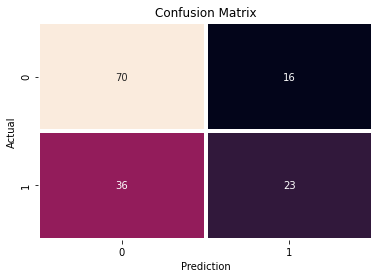
\includegraphics[width=0.5\textwidth]{figures/confusion_matrix.png}
    \caption{Contoh}
    \label{fig:my_label}
    \end{figure}
    dari confusion matrix tersebut, didapatkan
    \begin{itemize}
        \item TP = 70
        \item FP = 16
        \item TN = 36
        \item FN = 23
    \end{itemize}
    yang berarti total data prediksi benar yakni TP + FN = 70 + 23 = 93 data.
    oleh karenanya, akurasi bisa didapatkan dengan
\begin{lstlisting}
Akurasi = (TP + TN ) / (TP+FP+FN+TN) * 100%
Akurasi = 93/145*100%
Akurasi = 64%
\end{lstlisting}
\end{itemize}
\item Confusion Matrix\\
confusion matrix merupakan salah satu model klasifikasi yang digunakan untuk mengukur kinerja suatu model atau klasifikasi.\\
\par confusion matriks memberikan perbandingan hasil klasifikasi yang dihasilkan oleh model, dengan hasil klasifikasi yang sebenarnya dengan bentuk tabel matriks yang berisikan kombinasi nilai prediksi dan nilai aktual seperti berikut :
\begin{figure}[H]
    \centering
    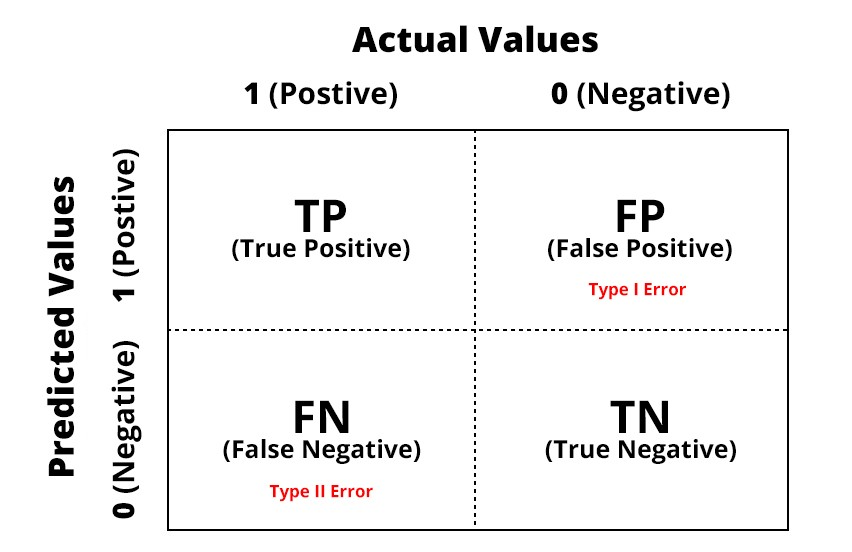
\includegraphics[width=0.50\textwidth]{figures/confusion_matriks.jpeg}
    \caption{Tabel Confusion Matriks}
    \label{fig:my_label}
\end{figure}
\par confusion matrix dibagi menjadi 2, yakni :
\begin{enumerate}
    \item binary classification confusion matrix \\
    ialah confusion matrix yang hanya memiliki 2 value pada label yang digunakan. contohnya ya/tidak, lulus/tidak lulus, baik/buruk, recommend/not recommend.
    \item multiclass classification confusion matrix\\
    ialah confusion matrix yang memiliki multiclass classification pada labelnya, yakni valuenya lebih dari 2. contohnya yaitu sangat buruk/buruk/baik/sangat baik, A/B/C/D/E, sangat tidak recommend/recommend/sangat recommend.
\end{enumerate}
berikut ini kode program untuk membuat visualisasi confusion matrix dengan matplotlib dan seaborn
\begin{lstlisting}
import pandas as pd, seaborn as sns, matplotlib.pyplot as plt, numpy as np
from sklearn.metrics import confusion_matrix
sns.heatmap(confusion_matrix(d_jeruk_test_pass, y_pred),annot=True,linewidths=3,cbar=False)
plt.title('Confusion Matrix')
plt.ylabel('Actual')
plt.xlabel('Prediction')
plt.show()
\end{lstlisting}
berikut ini contoh hasil confusion matrixnya :
\begin{enumerate}
    \item binary
    \begin{figure}[H]
    \centering
    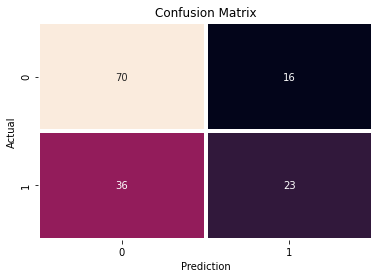
\includegraphics[width=0.75\textwidth]{figures/confusion_matrix.png}
    \caption{Hasil Visualisasi Binary Confusion Matriks}
    \label{fig:my_label}
    \end{figure}
    dari confusion matrix tersebut, didapatkan :
    \begin{itemize}
        \item TP = 70
        \item FP = 16
        \item TN = 36
        \item FN = 23
    \end{itemize}
    \item multiclass
    \begin{figure}[H]
    \centering
    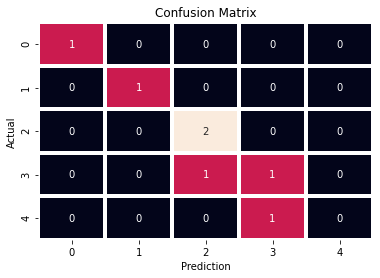
\includegraphics[width=0.75\textwidth]{figures/confusion_matrix2.png}
    \caption{Hasil Visualisasi Multiclass Confusion Matriks}
    \label{fig:my_label}
    \end{figure}
    Dari confusion matriks tersebut, didapat:
    \begin{itemize}
        \item Nilai actual dan nilai predict = 0 berjumlah 1 data
        \item Nilai actual dan nilai predict = 1 berjumlah 1 data
        \item Nilai actual dan nilai predict = 1 berjumlah 1 data
        \item Nilai actual dan nilai predict = 2 berjumlah 2 data
        \item Nilai actual = 3, namun nilai predict = 2 berjumlah 1 data
        \item Nilai actual dan nilai predict = 3, berjumlah 1 data
        \item Nilai actual = 4, namun nilai predict = 3 berjumlah 1 data
    \end{itemize}
Berikut hasil value metrics True Positive, False Positive, True Negative, dan False Negative dari confusion matrix di atas :
\begin{itemize}
    \item Huruf = 0 (A), memiliki representasi :
    \begin{enumerate}
        \item TP0 = 1
        \item FP0 = 0 + 0 + 0 + 0 = 0
        \item TN0 = 1 + 0 + 0 + 0 + 0 +2 + 0 + 0 +0 + 1+ 1 + 0 + 0 +0 + 1 + 0 = 6
        \item FN0  = 0 +0 +0 +0 = 0
    \end{enumerate}
    \item Huruf = 1 ( B), memiliki representasi :
    \begin{enumerate}
        \item TP1 = 1
        \item FP1 = 0 + 0 + 0 + 0 = 0
        \item TN1 = 1 + 0 + 0 + 0 + 0 +2 + 0 + 0 +0 + 1+ 1 + 0 + 0 +0 + 1 + 0 = 6
        \item FN1  = 0 +0 +0 +0 = 0
    \end{enumerate}
    \item Huruf = 2 ( C), memiliki representasi :
    \begin{enumerate}
        \item TP2 = 2
        \item FP2 = 0 + 0 + 0 + 0 = 0
        \item TN2 = 1 + (0*3) + 0 + 1 + (0*2) +(0*2) + 1 + 0 + (0*2) + 1 + 0 = 4
        \item FN2  = 0 +0 +1 +0 = 1
    \end{enumerate}
    \item Huruf = 3 ( D), memiliki representasi :
    \begin{enumerate}
        \item TP3 = 1
        \item FP3 = 0 + 0 + 1 + 0 = 1
        \item TN3 = 1 + (0*3) + 0 + 1 + (0*2) +(0*2) + 2 + (0*2) + (0*4) = 4
        \item FN3  = 0 +0 + 0 + 1 = 1
    \end{enumerate}
    \item Huruf = 4 ( huruf E), memiliki representasi :
    \begin{enumerate}
        \item TP4 = 0
        \item FP4 = 0 + 0 + 0 + 1 = 1
        \item TN4 = 1 + (0*3) + 0 + 1 + (0*2) +(0*2) + 2 + (0*2) + 1 + 1 = 6
        \item FN4  = 0 +0 + 0 + 0 = 0
    \end{enumerate}
\end{itemize}
\end{enumerate}
\item K-fold Cross Validation
Jelaskan bagaimana K-fold cross validation bekerja dengan gambar ilustrasi contoh buatan sendiri.\\
k-fold cross valdation ialah metode tambahan yang digunakan untuk dapat diperoleh hasil akurasi yang lebih maksimal. dinamakan k-fold cross validation karena dilakukan percobaan sebanyak k kali dengan menggunakan model dan parameter yang sama.\\
\par cross validation juga ialah teknik pengukuran vaidasi yang merupakan bentuk pengembangan dari model Split validation, yakni dilakukan dengan mengukur training error dengan melakukan uji menggunakan data testing.
berikut ini fungsi dari digunakannya k-fold cross validation, yakni :\\
\begin{enumerate}
    \item mengukur performa suatu model dengan melalui percobaan sebanyak k kali
    \item meningkatkan tingkat performansi model tersebut
    \item mengolah dataset dengan menggunakan kelas yang seimbang
    \item pengambilan sampel test yang lebih terstruktur
    \item menjangkau pengujian yang lebih efisien
\end{enumerate}
berikut ini contoh implementasi k-fold cross validation, seperti pada tabel berikut :
\begin{figure}[H]
    \centering
    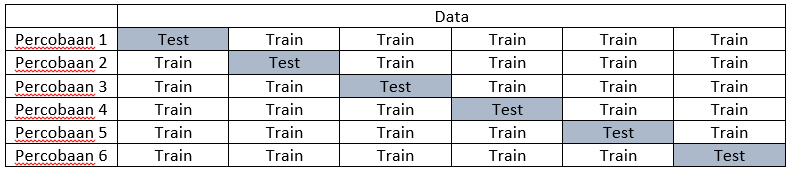
\includegraphics[width=0.75\textwidth]{figures/k-fold.png}
    \caption{contoh K-fold cross validation}
    \label{fig:my_label}
\end{figure}
dari contoh gambar di atas, dapat dibaca seperti berikut :
\begin{itemize}
    \item pada percobaan 1, data 1 digunakan untuk data testing, sisanya digunakan sebagai data training
    \item pada percobaan 2, data 2 digunakan untuk data testing, sisanya digunakan sebagai data training
    \item pada percobaan 3, data 3 digunakan untuk data testing, sisanya digunakan sebagai data training
    \item pada percobaan 4, data 4 digunakan untuk data testing, sisanya digunakan sebagai data training
    \item pada percobaan 5, data 5 digunakan untuk data testing, sisanya digunakan sebagai data training
    \item pada percobaan 6, data 6 digunakan untuk data testing, sisanya digunakan sebagai data training
\end{itemize}
sehingga, dapat disimpulkan bahwa, pada setiap percobaan testing validation selama k kali, data testing yang digunakan berbeda, begitu pula dengan data trainnya, sehingga memungkinkan agar semua data dapat dilakukan uji validasi supaya memaksimalkan akurasi dari model yang digunakan.
\item
Jelaskan apa itu decision tree dengan gambar ilustrasi contoh buatan sendiri.\\
Desicion tree ialah suatu model klasifikasi yang digunakan untuk melakukan pengambilan keputusan dengan menggunakan struktur pohon/hierarki.
metode ini menggabungkan 2 jenis pohon, yakni
\begin{enumerate}
    \item Classification tree
    \item Regression tree
\end{enumerate}
berikut ini contoh decision tree
\begin{figure}[H]
    \centering
    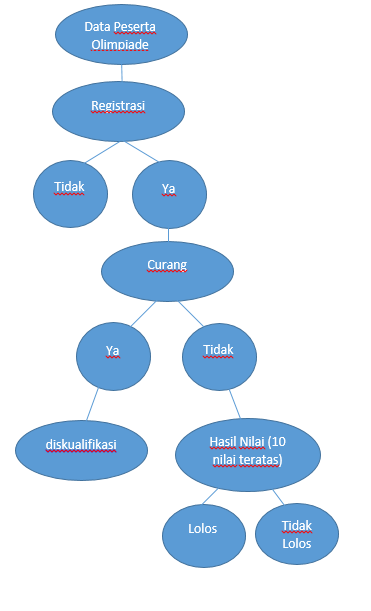
\includegraphics[width=0.75\textwidth]{figures/decisiontree.png}
    \caption{contoh decision dengan classification tree}
    \label{fig:my_label}
\end{figure}
\item Information Gain dan Entropy\\
\begin{enumerate}
    \item Information Gain\\
    Information Gain ialah salah satu metode yang digunakan untuk seleksi fitur, yakni mengukur efektifitas dari atribut yang digunakan dalam melakukan pengklasifikasian data.
    \item Entropy\\
    Entropy ialah suatu nilai yang berisikan informasi ukuran ketidakpastian (impurity) atribut dalam kumpulan objek data dalam satuan bit. semakin sedikit value dari atribut label, maka makin kecil pula nilai entropy yang dihasilkan. Sebaliknya, apabila nilai label multiclass, maka semakin besar pula nilai entropy yang dihasilkan.\\
    Contohnya, ketika dataset A dengan label yang bernilai positif dan negatif, dibandingkan dengan dataset B yang memiliki label tidak direkomensasi, direkomendasikan, dan sangat direkomendasikan. Maka, dari contoh tersebut, entropy dari dataset A lebih kecil dibandingkan dengan dataset B.
\begin{figure}[H]
    \centering
    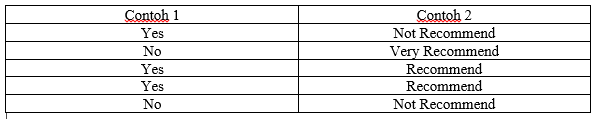
\includegraphics[width=0.75\textwidth]{figures/example.png}
    \caption{contoh atribut}
    \label{fig:my_label}
\end{figure}
dengan contoh tabel di atas, atribut contoh 1 akan memiliki nilai entropy yang lebih kecil dibandingkan dengan atribut contoh 2.
\end{enumerate}
\end{enumerate}

\section{ Praktikum Scikit-learn}
Dataset ambil di https://github.com/PacktPublishing/Python-Artificial-Intelligence-Projects-for-Beginners folder Chapter01.
Tugas anda adalah, dataset ganti menggunakan \textbf{student-mat.csv} dan mengganti semua nama variabel dari kode di bawah ini dengan nama-nama makanan (NPM mod 3=0), kota (NPM mod 3=1), buah (NPM mod 3=2), . Jalankan satu per satu kode tersebut di spyder dengan menggunakan textit{Run current cell}. Kemudian Jelaskan dengan menggunakan bahasa yang mudah dimengerti dan bebas plagiat dan wajib skrinsut dari komputer sendiri masing masing nomor di bawah ini(nilai 5 masing masing pada hari kedua).

\begin{enumerate}
\item
\begin{lstlisting}
# NPM = 1184030
# NPM%3
# import library pandas
import pandas as pd
# load dataset student-mat.csv
d_apel = pd.read_csv('student-mat.csv', sep=';')
# menghitung length dataset csv
len(d_apel)
# generate binary label (pass/fail) berdasar nilai G1+G2+G3, apabila total >= 35, maka bernilai 1, jika tidak maka 0
d_apel['pass'] = d_apel.apply(lambda row: 1 if (row['G1']+row['G2']+row['G3']) 
										>= 35 else 0, axis=1)
# drop row G1, G2 dan G3
d_apel = d_apel.drop(['G1', 'G2', 'G3'], axis=1)
# menampilkan 5 data teratas
d_apel.head()
# use one-hot encoding on categorical columns
d_apel = pd.get_dummies(d_apel, columns=['sex', 'school', 'address', 
								'famsize',
								'Pstatus', 'Mjob', 'Fjob', 'reason', 'guardian', 'schoolsup', 
								'famsup', 'paid', 'activities','nursery', 'higher', 'internet',
								'romantic'])
# menampilkan 5 data teratas
d_apel.head()
# shuffle rows
d_jeruk = d_apel.sample(frac=1)
# split training and testing data
d_jeruk_train = d_jeruk[:250]
d_jeruk_test = d_jeruk[250:]
# train atribut drop row pass
d_jeruk_train_att = d_jeruk_train.drop(['pass'], axis=1)
# train label menggunakan row pass
d_jeruk_train_pass = d_jeruk_train['pass']
# test atribut drop row pass
d_jeruk_test_att = d_jeruk_test.drop(['pass'], axis=1)
# test label menggunakan row pass
d_jeruk_test_pass = d_jeruk_test['pass']
# atribut drop row pass
d_jeruk_att = d_jeruk.drop(['pass'], axis=1)
# menggunakan row pass untuk label
d_jeruk_pass = d_jeruk['pass']

# import library
import numpy as np
# print number of passing students in whole dataset:
print("Passing: %d out of %d (%.2f%%)" % (np.sum(d_jeruk_pass), len(d_jeruk_pass), 
	       100*float(np.sum(d_jeruk_pass)) / len(d_jeruk_pass)))

# import library
from sklearn import tree
# instansiasi desicion tree classifier
melon = tree.DecisionTreeClassifier(criterion="entropy", max_depth=5)
# fit decision tree
melon = melon.fit(d_jeruk_train_att, d_jeruk_train_pass)
# import library graphviz untuk visualisasi
import graphviz
# instansiasi graphviz dari fit decision tree sebelumnya
mangga = tree.export_graphviz(melon, out_file=None, label="all", 
									impurity=False, proportion=True,
	                                feature_names=list(d_jeruk_train_att), 
									class_names=["fail", "pass"], 
	                                filled=True, rounded=True)
# buat variabel grafik visualisasi tree
graph = graphviz.Source(mangga)
# jalankan visualisasinya
graph
\end{lstlisting}
\item
\begin{lstlisting}
# save tree
tree.export_graphviz(melon, out_file="student-performance.dot", 
						 label="all", impurity=False, 
						 proportion=True,
	                     feature_names=list(d_train_att), 
	                     class_names=["fail", "pass"], 
	                     filled=True, rounded=True)
\end{lstlisting}
\item
\begin{lstlisting}
# cek score
melon.score(d_jeruk_test_att, d_jeruk_test_pass)
\end{lstlisting}
\item
\begin{lstlisting}
# import cross val score untuk cek cross validation score
from sklearn.model_selection import cross_val_score
# cek cross validation score
nangka_score = cross_val_score(melon, d_jeruk_att, d_jeruk_pass, cv=5)
# show average score and +/- two standard deviations away 
#(covering 95% of scores)
# print akurasi
print("Accuracy: %0.2f (+/- %0.2f)" % (nangka_score.mean(), nangka_score.std() * 2))
\end{lstlisting}
\item 
\begin{lstlisting}
# buat akurasi max depth
for max_depth in range(1, 20):
	    melon = tree.DecisionTreeClassifier(criterion="entropy", 
			max_depth=max_depth)
	    nangka_score = cross_val_score(melon, d_jeruk_att, d_jeruk_pass, cv=5)
	    print("Max depth: %d, Accuracy: %0.2f (+/- %0.2f)" % 
				(max_depth, nangka_score.mean(), nangka_score.std() * 2)
			 )
\end{lstlisting}
\item
\begin{lstlisting}
# buat akurasi depth acc
depth_acc = np.empty((19,3), float)
i = 0
for max_depth in range(1, 20):
    melon = tree.DecisionTreeClassifier(criterion="entropy", 
		max_depth=max_depth)
    nangka_score = cross_val_score(melon, d_jeruk_att, d_jeruk_pass, cv=5)
    depth_acc[i,0] = max_depth
    depth_acc[i,1] = nangka_score.mean()
    depth_acc[i,2] = nangka_score.std() * 2
    i += 1
# jalankan dept_acc
depth_acc
\end{lstlisting}
\item 
\begin{lstlisting}
	import matplotlib.pyplot as plt
	fig, ax = plt.subplots()
	ax.errorbar(depth_acc[:,0], depth_acc[:,1], yerr=depth_acc[:,2])
	plt.show()
\end{lstlisting}
\end{enumerate}


\section{Penanganan Error}
Dari percobaan yang dilakukan di atas, error yang kita dapatkan di dokumentasikan dan di selesaikan(nilai 5 hari kedua):
\begin{enumerate}
	\item Screenshoot Error
\begin{figure}[H]
    \centering
    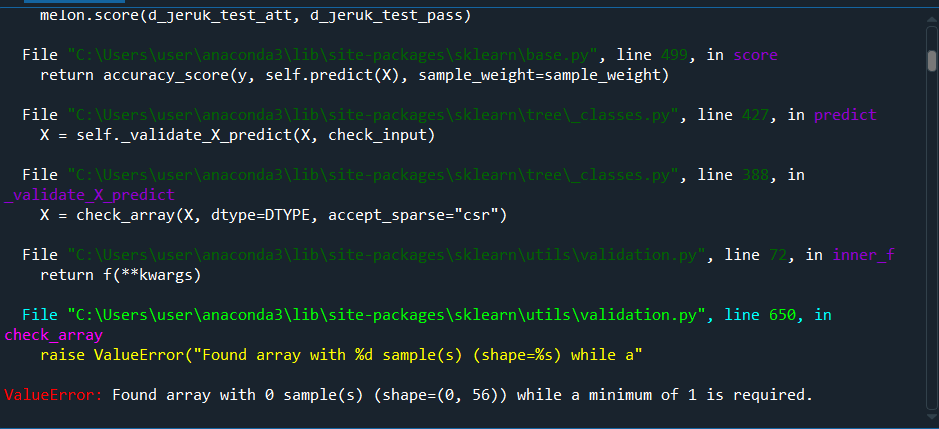
\includegraphics[width=1\textwidth]{figures/Screenshot (2341).png}
    \caption{Error}
    \label{fig:my_label}
\end{figure}
	\item
Kode eror dan jenis errornya\\
\begin{lstlisting}
ValueError: Found array with 0 sample(s) (shape=(0, 56)) while a minimum of 1 is required.
\end{lstlisting}
	\item Solusi pemecahan masalah error\\
solusi yang dilakukan ialah dengan melakukan pengecekan kembali terhadap data yang ditest dan ditrain, di source code yang sebelumnya, digunakan 500 data awal pada data train, dan setelah 500 data awal di data test, namun pada praktikum kali ini, data yang digunakan bahkan tidak lebih dari 500, melainkan hanya 395. sehingga memunculkan error tersebut.
sehingga solusinya yakni mengubah banyak data yang displit untuk data train dan data test dengan menyesuaikan jumlah datanya, disini saya mengubah menjadi 250 data awal untuk data training, dan sisanya untuk data testingnya
\end{enumerate}